% Mengatur spasi antar elemen
\setlength{\parskip}{0pt} % Jarak antar paragraf
\setlength{\baselineskip}{1.2\baselineskip} % Jarak antar baris
\setlength{\parindent}{1em} % Indentasi awal paragraf
\setlength{\intextsep}{0pt} % Jarak atas dan bawah gambar
\setlength{\abovecaptionskip}{1pt} % Jarak gambar dan caption
\setlength{\belowcaptionskip}{1pt} % Jarak caption dan teks

\raggedbottom % Hindari perataan otomatis halaman



\chapter{METODOLOGI}

\section{Metode yang Digunakan}
Penelitian ini bertujuan untuk merancang dan mengimplementasikan sistem minting NFT berbasis \textit{Solana Blockchain} untuk tiket konser musik dengan memanfaatkan teknologi \textit{Web3.0}. Diagram alur metodologi penelitian ditampilkan pada Gambar \ref{fig:metodologi-penelitian}.

% Tambahkan diagram metodologi penelitian
\begin{figure}[H]
    \centering
    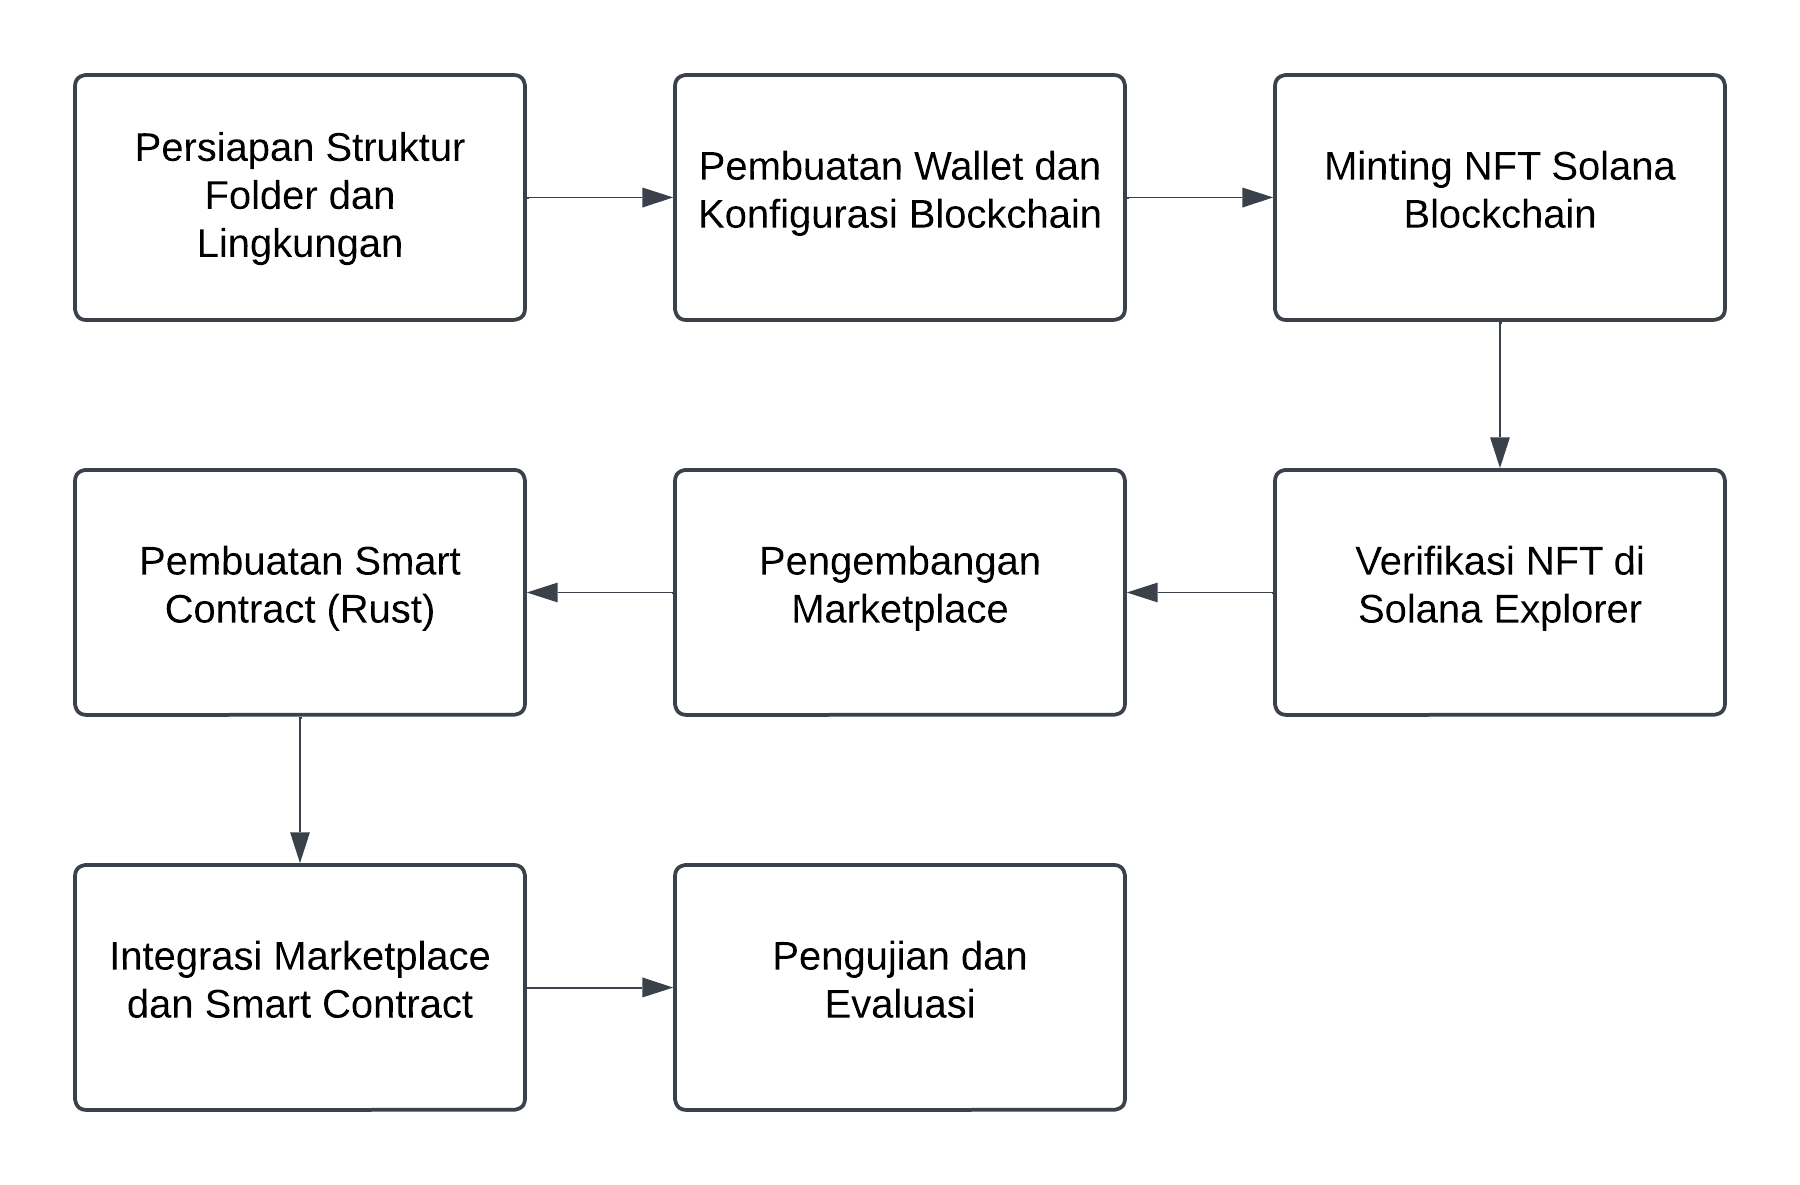
\includegraphics    {gambar/Diagram3.1.png}
    \caption{Metodologi Penelitian yang Digunakan}
    \label{fig:metodologi-penelitian}
\end{figure}

\section{Tahapan Implementasi}
Tahapan dalam penelitian ini meliputi beberapa langkah sistematis yang dirancang untuk mengembangkan sistem minting NFT berbasis \textit{Solana Blockchain}. Setiap tahapan mencakup langkah-langkah teknis mulai dari persiapan lingkungan pengembangan hingga implementasi dan pengujian sistem.

\subsection{Persiapan Lingkungan dan Struktur Folder}
Langkah pertama dalam penelitian ini adalah menyiapkan struktur folder proyek yang terorganisir untuk mempermudah pengelolaan kode dan sumber daya proyek. Struktur folder yang dibuat adalah sebagai berikut:

\begin{enumerate}
    \item {backend:} Berisi konfigurasi wallet, script untuk mengelola proses minting NFT, dan fungsi backend lainnya.
    \item {frontend:} Mengimplementasikan \textit{Next.js} untuk antarmuka pengguna yang mendukung integrasi Web3.0.
    \item {metadata:} Menyimpan file \textit{JSON} yang berisi deskripsi dan atribut NFT tiket konser.
    \item {images:} Menyimpan gambar atau media pendukung NFT yang akan digunakan dalam metadata.
    \item {scripts:} Berisi kode-kode otomasi seperti script untuk melakukan minting dan verifikasi NFT.
\end{enumerate}

Untuk mendukung pengembangan sistem, beberapa dependensi utama diinstal pada proyek ini, antara lain:
\begin{enumerate}
    \item \textit{}{@solana/web3.js}: Untuk menghubungkan dan berinteraksi dengan blockchain Solana.
    \item \textit{@metaplex-foundation/js}: Untuk mendukung proses minting NFT menggunakan Metaplex SDK.
    \item \textit{dotenv}: Untuk mengelola variabel lingkungan seperti \textit{private key} dan konfigurasi RPC URL.
    \item \textit{@solana/wallet-adapter-react} dan \textit{@solana/wallet-adapter-react-ui}: Untuk integrasi dengan \textit{Phantom Wallet} pada antarmuka pengguna.
\end{enumerate}

Selain itu, file konfigurasi \texttt{.env} disiapkan untuk menyimpan informasi sensitif, seperti RPC URL Devnet Solana dan alamat wallet. Gambar \ref{fig:folder-structure} menunjukkan struktur folder yang digunakan dalam proyek ini.

\begin{figure}[H]
    \centering
    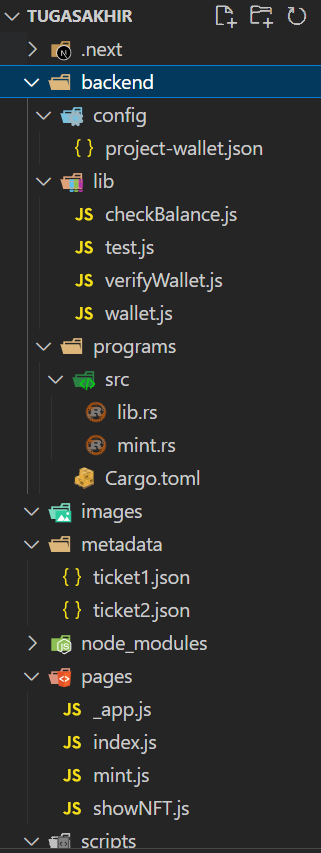
\includegraphics[width=0.2\textwidth]{gambar/3.2.1.png}
    \caption{Struktur Folder Proyek}
    \label{fig:folder-structure}
\end{figure}

Dengan struktur folder yang terorganisir, pengelolaan proyek menjadi lebih mudah, baik dalam pengembangan backend, frontend, maupun pengelolaan sumber daya pendukung seperti metadata dan gambar.

\subsection{Persiapan Lingkungan Pengembangan}
Langkah berikutnya adalah mengatur lingkungan pengembangan untuk memastikan sistem berjalan dengan baik. Langkah-langkah ini meliputi:
\begin{enumerate}
    \item Instalasi dependensi proyek menggunakan \textit{npm install}.
    \item Konfigurasi wallet Solana menggunakan \textit{solana-keygen new} untuk membuat wallet baru dan menyimpan \textit{keypair} pada folder \textit{backend/config}.
    \item Menentukan RPC URL yang akan digunakan, yaitu Solana Devnet, menggunakan perintah \textit{solana config set --url https://api.devnet.solana.com}.
\end{enumerate}

Dengan persiapan lingkungan pengembangan yang matang, sistem dapat mendukung implementasi proses minting NFT, integrasi frontend dengan wallet, dan pengujian yang terorganisir.


\subsection{Pembuatan Wallet Solana}

Tahap pembuatan wallet Solana merupakan langkah awal dalam membangun sistem berbasis blockchain yang mendukung proses minting NFT. Wallet ini bertugas untuk menyimpan kunci privat dan publik yang diperlukan dalam proses transaksi pada jaringan Solana. Wallet juga bertindak sebagai identitas pengguna di jaringan blockchain, memungkinkan pengguna untuk mengakses dan mengelola NFT mereka. Proses dimulai dengan menggunakan perintah \textit{solana-keygen new} untuk membuat \textit{keypair}, yang berisi kunci privat dan kunci publik. File \textit{keypair} yang dihasilkan kemudian disimpan pada folder \textit{config}, memastikan pengelolaan yang terorganisir dan keamanan akses. Kunci privat dalam file ini penting untuk menandatangani transaksi blockchain, sementara kunci publik digunakan untuk mengidentifikasi akun wallet pada jaringan Solana.

Selanjutnya, konfigurasi RPC (Remote Procedure Call) Solana dilakukan dengan menggunakan perintah \textit{solana config set --url https://api.devnet.solana.com}. RPC Devnet dipilih karena mendukung pengujian dan pengembangan aplikasi tanpa memerlukan aset asli pada jaringan utama (Mainnet). Dengan konfigurasi ini, wallet yang dibuat terhubung dengan Devnet, memungkinkan pengguna untuk menguji transaksi, seperti minting NFT, dalam lingkungan yang aman dan bebas biaya. Melalui langkah-langkah ini, wallet Solana berhasil disiapkan sebagai elemen penting dalam sistem, mendukung koneksi ke blockchain dan berfungsi sebagai tempat penyimpanan serta alat transaksi dalam pengelolaan tiket konser berbasis NFT.

\subsection{Proses Minting NFT}

Proses \textit{minting} NFT merupakan inti dari penelitian ini. Pada tahap ini, tiket konser digital berbasis \textit{blockchain} dibuat melalui beberapa langkah utama, yakni pembuatan metadata, pengunggahan metadata ke \textit{IPFS}, dan pencetakan NFT ke jaringan Solana menggunakan \textit{Metaplex SDK}. Tahapan ini memastikan NFT yang dihasilkan terintegrasi dengan sistem \textit{blockchain} serta memiliki metadata yang lengkap dan valid.

Langkah pertama dalam proses ini adalah pembuatan \textit{metadata}. \textit{Metadata} merupakan deskripsi terstruktur dari NFT yang mencakup elemen-elemen penting seperti nama tiket (\textit{title}), deskripsi tiket (\textit{description}), dan URL gambar tiket (\textit{image}). \textit{Metadata} ini disimpan dalam file JSON yang dirancang untuk menyimpan data secara konsisten dan mudah digunakan selama proses \textit{minting}.

Langkah berikutnya adalah mengunggah \textit{metadata} ke \textit{IPFS} (\textit{InterPlanetary File System}). \textit{IPFS} adalah sistem penyimpanan terdesentralisasi yang digunakan untuk menyimpan data secara permanen dengan jaminan integritas dan keamanan. Penelitian ini menggunakan layanan Pinata untuk mengunggah file JSON \textit{metadata}. Setelah file berhasil diunggah, Pinata menghasilkan \textit{Content Identifier} (\textit{CID}), yaitu sebuah pengenal unik yang memungkinkan \textit{metadata} dapat diakses kapan saja melalui jaringan \textit{IPFS}.

Langkah terakhir dalam proses ini adalah pencetakan NFT menggunakan \textit{Metaplex SDK}. Dengan pustaka Metaplex, \textit{minting} NFT dapat dilakukan melalui fungsi bawaan seperti \textit{metaplex.nfts().create()}. Fungsi ini membutuhkan \textit{metadata} yang telah disiapkan sebelumnya serta \textit{wallet} Solana untuk mengeksekusi proses \textit{minting} di \textit{blockchain}. Proses ini menghasilkan NFT dengan \textit{metadata} yang terhubung ke \textit{IPFS}, sehingga informasi tiket tersimpan secara aman dan dapat diverifikasi. Berikut adalah kode implementasi:

\begin{verbatim}[language=JavaScript, caption=Proses Minting NFT dengan Metaplex SDK]
const nft = await metaplex.nfts().create({
    uri: "https://gateway.pinata.cloud/ipfs/{CID}",
    name: "VIP Concert Ticket",
    symbol: "VIPT",
    sellerFeeBasisPoints: 500,
    maxSupply: 1,
});
console.log("NFT berhasil dimint:", nft.mintAddress.toString());
\end{verbatim}

Proses ini dapat dilihat pada Gambar \ref{fig:minting-nft}, yang menunjukkan alur \textit{minting NFT} mulai dari pembuatan \textit{metadata} hingga pencetakan tiket digital di \textit{blockchain} Solana.

\begin{figure}[H]
    \centering
    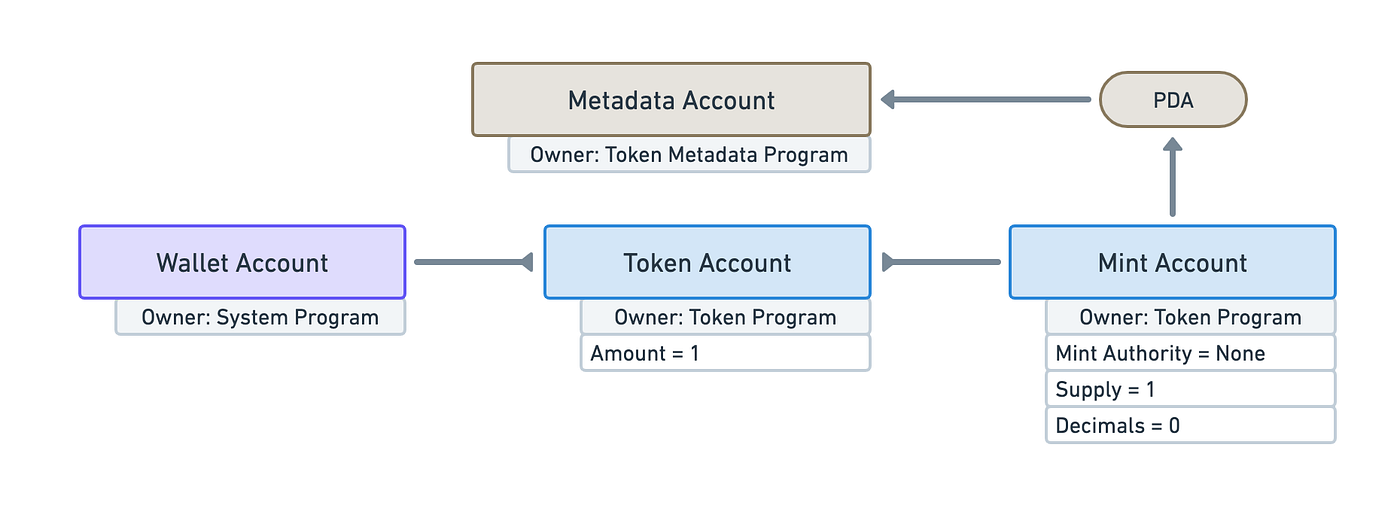
\includegraphics[scale=0.3]{gambar/3.2.2.png}
    \caption{Proses Minting NFT}
    \label{fig:minting-nft}
\end{figure}

Tahapan ini menghasilkan tiket konser berbasis NFT yang aman dan sesuai standar. Penggunaan \textit{IPFS} untuk penyimpanan \textit{metadata} dan integrasi dengan \textit{blockchain} Solana menjamin bahwa NFT yang dihasilkan memiliki validitas, keamanan, dan dapat digunakan pada \textit{marketplace} atau sistem berbasis \textit{Web3.0}.



% ====================
% Bagian Integrasi Frontend dengan Wallet
% ====================
\subsection{Integrasi Frontend dengan Wallet}
Integrasi \textit{wallet} dengan aplikasi frontend merupakan komponen kritis dalam sistem NFT \textit{ticketing}. \textit{Phantom Wallet} dipilih sebagai \textit{wallet} utama karena popularitasnya di ekosistem Solana dan fitur-fitur keamanan yang ditawarkannya. Proses integrasi menggunakan library \textit{@solana/wallet-adapter-react} yang menyediakan hooks dan komponen React untuk berinteraksi dengan \textit{Phantom Wallet} \parencite{ref5}.

Dalam implementasinya, aplikasi menggunakan \textit{WalletProvider} untuk menyediakan konteks wallet ke seluruh aplikasi:

\begin{verbatim}
const WalletContextProvider = ({ children }) => {
 const wallets = useMemo(
   () => [
     new PhantomWalletAdapter(),
   ],
   []
 );

 return (
   <ConnectionProvider endpoint={endpoint}>
     <WalletProvider wallets={wallets}>
       {children}
     </WalletProvider>
   </ConnectionProvider>
 );
};
\end{verbatim}

Antarmuka pengguna untuk proses \textit{minting} tiket dirancang dengan mempertimbangkan pengalaman pengguna dan keamanan. Komponen utama termasuk tombol "Mint NFT" yang memanggil \textit{smart contract} di Solana melalui transaksi yang ditandatangani oleh \textit{wallet} pengguna. Proses ini melibatkan beberapa tahap:

\begin{enumerate}
   \item Koneksi \textit{wallet}: Memastikan pengguna telah terhubung dengan \textit{Phantom Wallet}
   \item Verifikasi saldo: Memeriksa apakah pengguna memiliki cukup SOL untuk transaksi
   \item Pembuatan transaksi: Menyiapkan instruksi untuk \textit{minting} NFT
   \item Penandatanganan: Meminta persetujuan pengguna melalui \textit{wallet}
   \item Konfirmasi: Menunggu konfirmasi transaksi dari jaringan Solana
\end{enumerate}

Keamanan transaksi dijamin melalui implementasi beberapa mekanisme:
\begin{enumerate}
   \item Validasi input pengguna sebelum membuat transaksi
   \item Pengecekan status koneksi \textit{wallet} secara berkala
   \item Penanganan error yang komprehensif
   \item Feedback real-time kepada pengguna selama proses transaksi
\end{enumerate}

\begin{figure}[H]
   \centering
   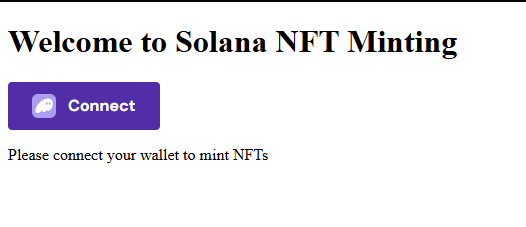
\includegraphics[width=0.9\textwidth]{gambar/3.2.3.png}
   \caption{Arsitektur Integrasi Wallet dengan Frontend \parencite{ref5}}
   \label{fig:wallet-integration}
\end{figure}


\subsection{Pengujian dan Verifikasi}
Proses pengujian dan verifikasi bertujuan untuk memastikan bahwa sistem \textit{minting NFT} untuk tiket konser musik berbasis \textit{Solana Blockchain} berfungsi sesuai dengan spesifikasi yang telah dirancang. Pengujian ini melibatkan berbagai tahapan, mulai dari validasi metadata NFT hingga integrasi sistem secara keseluruhan.

Tahapan pertama adalah pengujian metadata NFT yang disimpan dalam format \textit{JSON}. Metadata diverifikasi untuk memastikan informasi seperti nama tiket, deskripsi, dan URL gambar yang diunggah ke \textit{IPFS} sudah lengkap dan sesuai standar. Proses ini juga mencakup pengujian koneksi ke \textit{IPFS}, memastikan file metadata dapat diakses menggunakan \textit{Content Identifier (CID)} yang dihasilkan oleh layanan seperti \textit{Pinata}.
\begin{figure}[H]
    \centering
    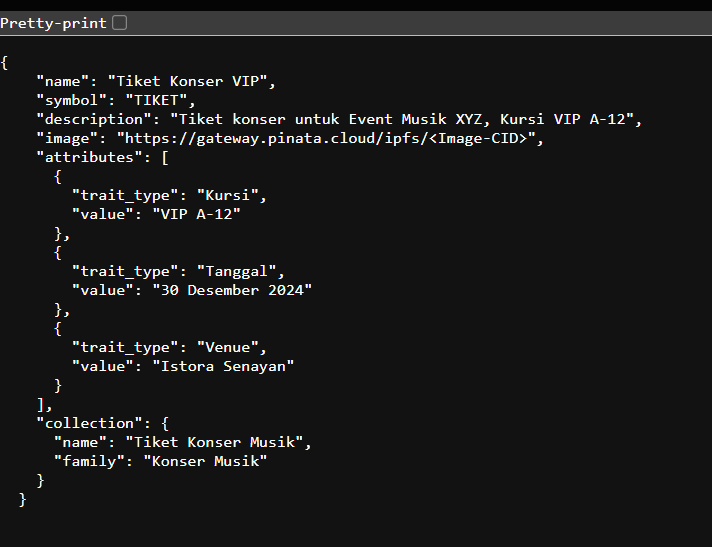
\includegraphics[width=0.7\textwidth]{gambar/3.2.4.png}
    \caption{Metadata Tiket Konser VIP dalam Format JSON}
    \label{fig:metadata-json}
\end{figure}
Setelah metadata JSON untuk tiket konser dibuat, langkah selanjutnya adalah mengunggah file metadata tersebut ke sistem penyimpanan terdesentralisasi menggunakan layanan \textit{Pinata}. Pinata memungkinkan pengguna untuk menyimpan metadata pada jaringan \textit{IPFS (InterPlanetary File System)} dan menghasilkan \textit{Content Identifier (CID)}, yaitu sebuah pengenal unik untuk file yang diunggah. CID ini digunakan sebagai URI untuk metadata dalam proses minting NFT.

\begin{figure}[H]
    \centering
    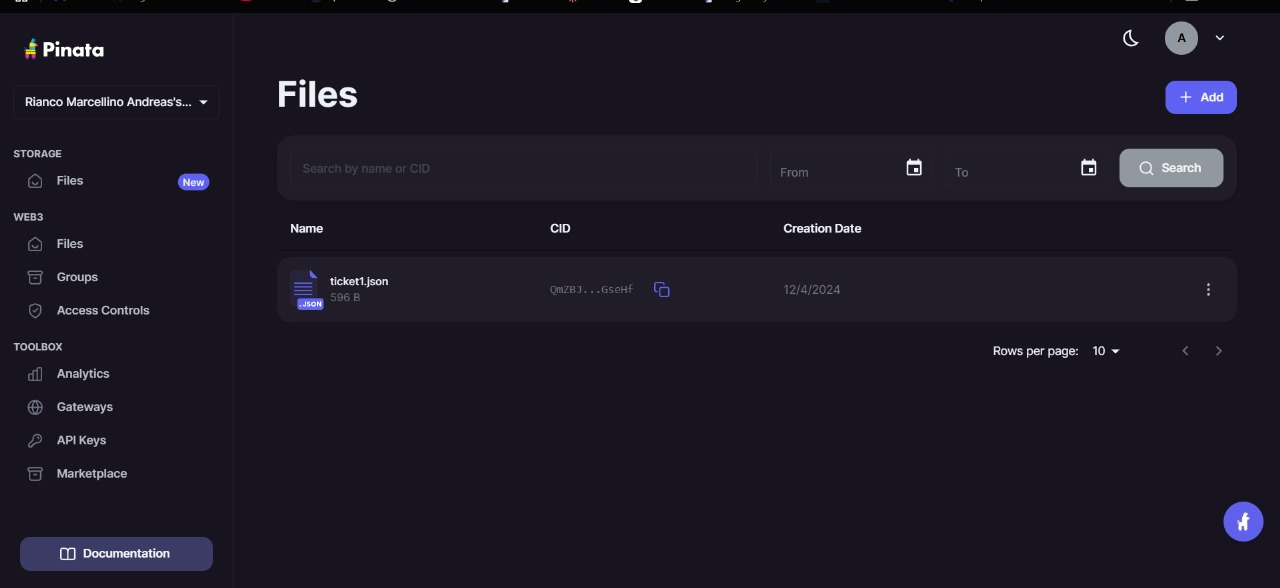
\includegraphics[width=1\textwidth]{gambar/3.2.7.jpg}
    \caption{Antarmuka Pinata untuk Metadata JSON}
    \label{fig:pinata-interface}
\end{figure}

Gambar \ref{fig:pinata-interface} menunjukkan tampilan antarmuka Pinata, di mana file JSON metadata tiket konser berhasil diunggah dan \textit{CID} yang dihasilkan dapat dilihat. \textit{CID} ini digunakan dalam langkah berikutnya untuk mencetak NFT pada jaringan blockchain Solana.

Tahapan berikutnya adalah pengujian proses \textit{minting} NFT. Proses ini dilakukan menggunakan fungsi dari \textit{Metaplex SDK}, yang mencakup pembuatan akun token, pengaturan metadata, dan pencetakan tiket digital di jaringan \textit{Solana}. Pengujian dilakukan untuk memastikan bahwa NFT tercatat pada blockchain dengan metadata yang sesuai. Selain itu, hasil minting diverifikasi melalui \textit{Solana Explorer} untuk memeriksa apakah NFT berhasil ditambahkan ke akun pengguna.

\begin{figure}[H]
    \centering
    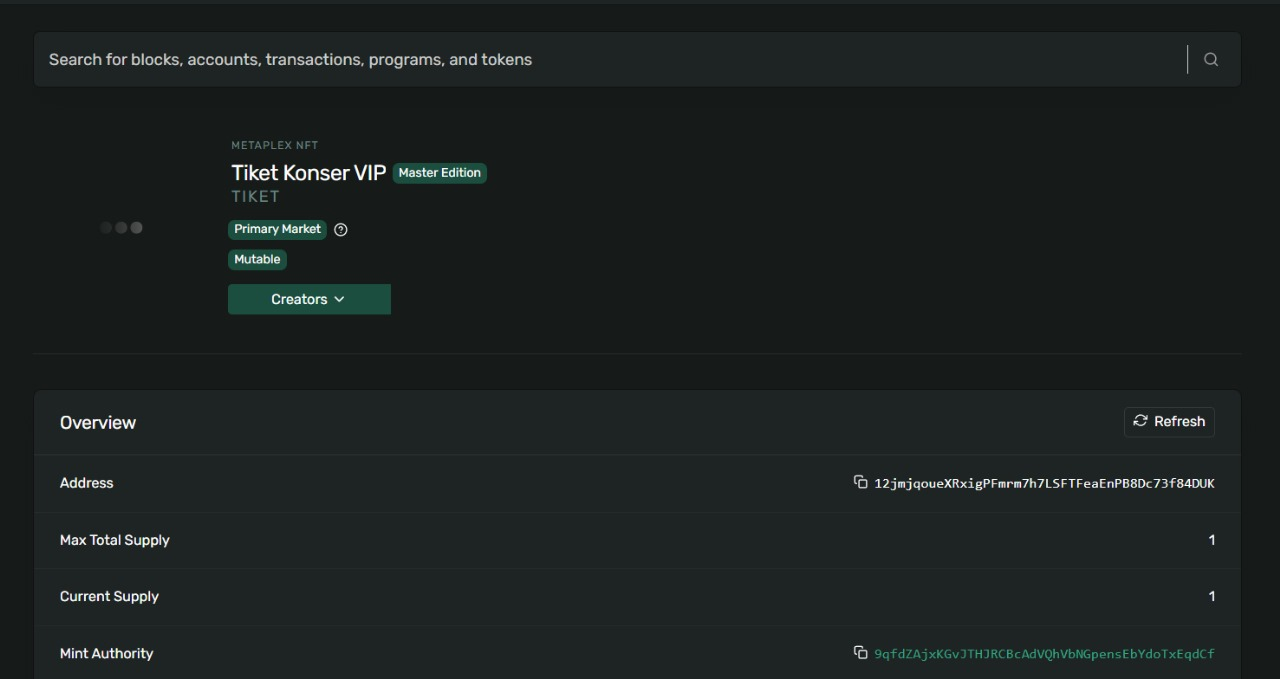
\includegraphics[width=1\textwidth]{gambar/3.2.5}
    \caption{Verifikasi NFT di Solana Explorer}
    \label{fig:solana-explorer}
\end{figure}
Pengujian juga mencakup integrasi antarmuka pengguna dengan \textit{Phantom Wallet}. Proses ini melibatkan koneksi \textit{wallet}, validasi saldo, penandatanganan transaksi, dan konfirmasi transaksi di jaringan \textit{Solana}. Hasil pengujian menunjukkan bahwa \textit{Phantom Wallet} dapat terhubung dengan aplikasi tanpa hambatan, dan transaksi \textit{minting} dapat diselesaikan dengan sukses. 


Pengujian menyeluruh (\textit{end-to-end}) dilakukan untuk memverifikasi integrasi antara \textit{frontend}, \textit{backend}, dan blockchain. Pengguna dapat menghubungkan \textit{wallet}, melakukan proses \textit{minting}, dan memverifikasi tiket konser mereka melalui antarmuka pengguna yang telah dirancang. Selain itu, pengujian ini memastikan bahwa NFT yang dihasilkan kompatibel dengan \textit{marketplace} berbasis \textit{Solana}, sehingga dapat digunakan untuk transaksi lebih lanjut. 

Hasil pengujian menunjukkan bahwa sistem \textit{minting NFT} berjalan dengan baik dalam lingkungan pengujian. Metadata NFT dapat diakses melalui \textit{IPFS}, transaksi pada blockchain \textit{Solana} berhasil tercatat, dan antarmuka pengguna memberikan pengalaman yang mulus serta aman bagi pengguna. Hal ini memastikan bahwa sistem telah siap digunakan untuk pengelolaan tiket konser berbasis \textit{Web3.0}.

\section{Pengembangan Smart Contract untuk Minting NFT}

Smart contract dalam penelitian ini dikembangkan menggunakan bahasa pemrograman \textit{Rust} dengan memanfaatkan \textit{Solana Program Library (SPL)}. Smart contract dirancang untuk mendukung proses \textit{minting NFT} tiket konser berbasis \textit{Solana Blockchain}. Dengan memanfaatkan SPL, pengembangan menjadi lebih efisien karena tersedia fungsi-fungsi bawaan yang mendukung berbagai operasi pada blockchain Solana.

\subsection{Fungsi Utama Smart Contract}
Smart contract memiliki dua fungsi utama yang diimplementasikan, yaitu:

\begin{enumerate}
    \item \textit{Minting NFT}: Fungsi ini bertanggung jawab untuk menciptakan NFT baru berdasarkan metadata yang telah disiapkan. Metadata mencakup elemen-elemen seperti nama tiket, deskripsi, gambar, dan atribut tambahan yang disimpan di \textit{IPFS}.
    \item \textit{Validasi Tiket}: Fungsi ini memastikan setiap tiket yang telah dicetak hanya dapat digunakan oleh satu pengguna. Validasi ini mencegah terjadinya penggunaan tiket yang sama oleh beberapa pengguna atau penggunaan tidak sah.
\end{enumerate}

\subsection{Proses Implementasi Smart Contract}
Implementasi smart contract melibatkan beberapa langkah penting:

Pengembangan Fungsi Minting
Fungsi \textit{mint} adalah inti dari smart contract. Fungsi ini memungkinkan pengguna mencetak NFT baru berdasarkan metadata yang telah diunggah ke \textit{IPFS}. Kode berikut menunjukkan contoh implementasi fungsi \textit{mint}:

\begin{verbatim}
pub fn mint_token(
    ctx: Context<MintToken>,
    metadata_uri: String,
) -> ProgramResult {
    let mint = &mut ctx.accounts.mint;
    let metadata = &mut ctx.accounts.metadata;
    let owner = &mut ctx.accounts.owner;

    // Assign metadata URI to token
    metadata.uri = metadata_uri;

    // Mint token to owner
    mint.owner = *owner.key;
    mint.supply = 1;

    Ok(())
}
\end{verbatim}

Validasi Metadata
Smart contract memverifikasi metadata yang disertakan dalam proses minting. Metadata diverifikasi untuk memastikan keaslian data dan kompatibilitas dengan standar NFT di Solana. Elemen-elemen penting seperti \textit{name}, \textit{symbol}, dan \textit{attributes} dipastikan sudah sesuai dengan tiket konser.

Validasi Tiket
Fungsi validasi memastikan bahwa setiap tiket hanya dapat digunakan oleh satu pengguna. Proses validasi dilakukan dengan menyimpan informasi pemilik tiket pada akun token terkait. Setiap kali tiket digunakan, status kepemilikan diperiksa untuk mencegah penggunaan ganda.

\subsection{Keamanan dan Pengujian Smart Contract}
Pengembangan smart contract juga mencakup pengujian dan penerapan langkah-langkah keamanan sebagai berikut:

\begin{enumerate}
    \item {Pemeriksaan Input}: Setiap data input ke dalam smart contract diverifikasi untuk memastikan kesesuaian dengan format dan standar yang ditetapkan.
    \item {Penanganan Error}: Smart contract dirancang untuk menangani berbagai skenario error, seperti kegagalan transaksi atau ketidakcocokan metadata.
    \item {Pengujian Unit}: Fungsi-fungsi dalam smart contract diuji menggunakan framework \textit{Anchor} untuk memastikan logika berjalan sesuai dengan desain.
\end{enumerate}

\subsection{Hasil Implementasi dan Integrasi}
Hasil implementasi menunjukkan bahwa smart contract berhasil melakukan minting NFT berdasarkan metadata yang telah disiapkan. Tiket konser yang dihasilkan dapat diverifikasi pada blockchain Solana melalui Solana Explorer atau dompet digital seperti \textit{Phantom Wallet}. Integrasi dengan frontend menggunakan \textit{Anchor} dan \textit{@solana/web3.js} memastikan bahwa pengguna dapat dengan mudah mengakses fungsi-fungsi yang ada dalam smart contract.

\begin{figure}[H]
    \centering
    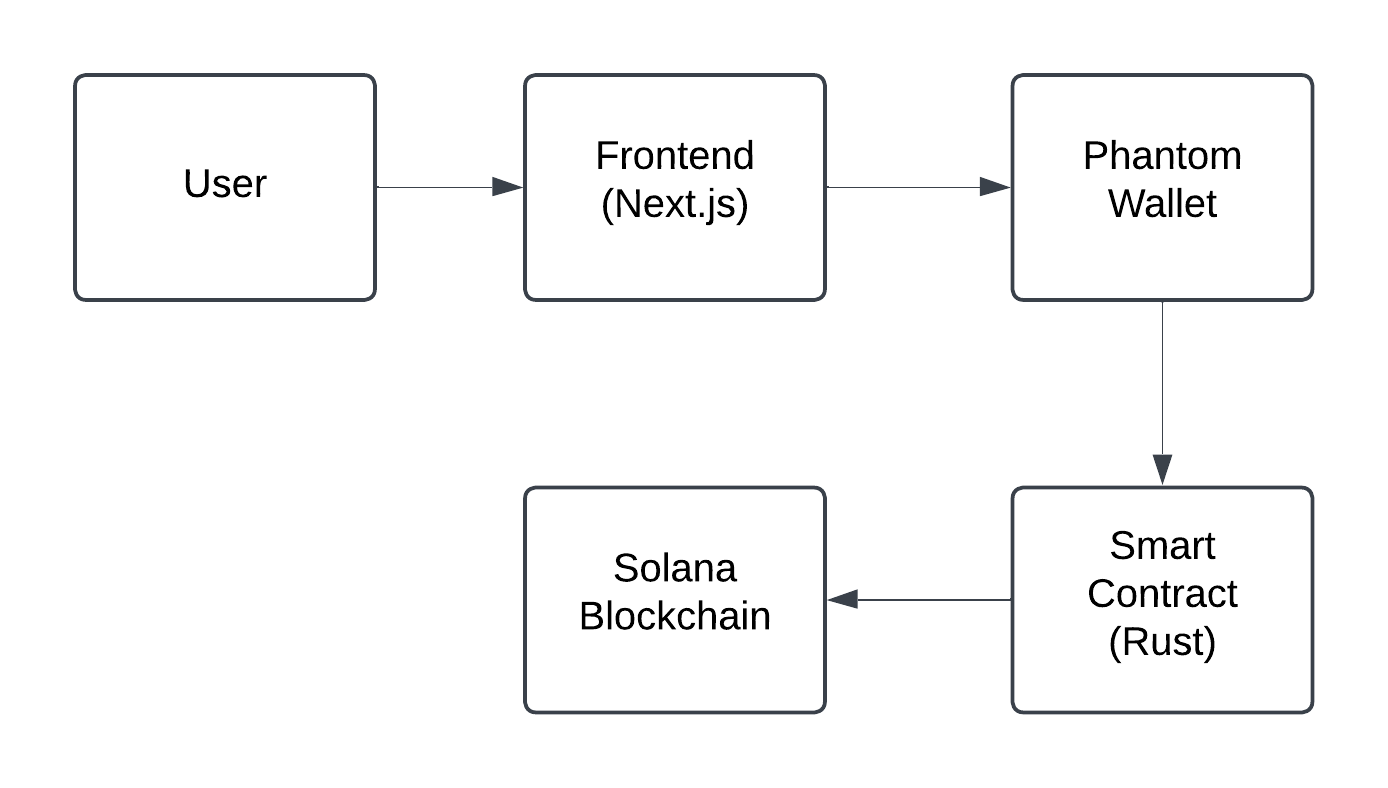
\includegraphics[scale=1]{gambar/3.2.6.png}
    \caption{Arsitektur Smart Contract untuk Minting NFT}
    \label{fig:smart-contract-architecture}
\end{figure}

Dengan implementasi ini, sistem minting NFT untuk tiket konser musik berbasis blockchain tidak hanya efisien tetapi juga aman dan dapat diandalkan. Smart contract yang dikembangkan mendukung standar NFT pada Solana dan memungkinkan integrasi dengan marketplace berbasis \textit{Web3.0}.


\section{Pembuatan Marketplace NFT untuk Tiket Konser}

Marketplace NFT untuk tiket konser dikembangkan menggunakan teknologi \textit{Web3.0} dengan memanfaatkan \textit{Next.js} sebagai kerangka kerja frontend. Platform ini dirancang untuk mendukung transaksi tiket konser berbasis blockchain yang memungkinkan pengguna untuk menjual, membeli, dan mengelola tiket mereka secara terdesentralisasi. Dengan integrasi blockchain Solana, marketplace ini memastikan bahwa setiap transaksi dilakukan secara aman, transparan, dan efisien.

Salah satu fitur utama dari marketplace ini adalah kemampuan pengguna untuk menampilkan tiket NFT mereka untuk dijual. Proses ini melibatkan pencantuman metadata NFT, seperti nama tiket, deskripsi, harga, dan atribut lainnya yang ditampilkan secara langsung pada halaman listing. Pengguna dapat dengan mudah mengunggah tiket mereka melalui antarmuka yang ramah pengguna.

Selain itu, marketplace juga menyediakan fitur pembelian tiket. Pengguna lain dapat membeli tiket yang tersedia dengan menggunakan mata uang digital SOL. Transaksi ini dilakukan secara otomatis melalui \textit{smart contract}, yang memastikan bahwa pembayaran dilakukan sebelum transfer kepemilikan NFT. Proses pembelian dirancang untuk meminimalkan risiko penipuan dan memberikan pengalaman yang aman bagi semua pengguna.

Fitur penting lainnya adalah transfer kepemilikan tiket. Setelah transaksi pembelian berhasil, kepemilikan NFT secara otomatis dipindahkan dari penjual ke pembeli. Proses ini dilakukan melalui blockchain Solana, sehingga setiap perubahan status kepemilikan tercatat secara permanen dan dapat diverifikasi oleh semua pihak. Dengan demikian, marketplace ini mendukung model transaksi terdesentralisasi yang efisien dan dapat dipercaya.

Marketplace ini berfungsi sebagai solusi inovatif untuk pengelolaan tiket konser berbasis NFT, memanfaatkan teknologi blockchain untuk menghadirkan keaslian, keamanan, dan efisiensi dalam ekosistem tiket digital.



